% THIS TEMPLATE IS A WORK IN PROGRESS

\documentclass{article}
\usepackage{graphicx}
\usepackage{hyperref}
\usepackage{fancyhdr}
\usepackage{float}
\usepackage{hyperref}
\usepackage{mathtools}
\usepackage{caption}
\usepackage{subcaption}

% FOR CODE
\usepackage{listings}
\usepackage{xcolor}
\usepackage{xparse}
\NewDocumentCommand{\codeword}{v}{%
\texttt{{#1}}%
}

\definecolor{codegreen}{rgb}{0,0.6,0}
\definecolor{codegray}{rgb}{0.5,0.5,0.5}
\definecolor{codepurple}{rgb}{0.58,0,0.82}
\definecolor{backcolour}{rgb}{0.95,0.95,0.92}

\lstdefinestyle{mystyle}{
    backgroundcolor=\color{backcolour},   
    commentstyle=\color{codegreen},
    keywordstyle=\color{magenta},
    numberstyle=\tiny\color{codegray},
    stringstyle=\color{codepurple},
    basicstyle=\ttfamily\footnotesize,
    breakatwhitespace=false,         
    breaklines=true,                 
    captionpos=b,                    
    keepspaces=true,                 
    numbers=left,                    
    numbersep=5pt,                  
    showspaces=false,                
    showstringspaces=false,
    showtabs=false,                  
    tabsize=2
}

\lstset{style=mystyle}
% 

\fancypagestyle{firstpage}{%
  \lhead{CAP6610 Project Progress Report}
  \rhead{Akash Gajjar}
}

\begin{document}
\thispagestyle{firstpage}

\section{Summary}

Previously the GAN that I was trying to implement was from a different paper \cite{1} in which they used convolutional neural networks to implement GAN. Since the GAN architecture proposed in the original paper was very different \cite{2}, I implemented the model inspired by the original paper in order to be able to fairly compare the results with VAE. First I created the Generator and Discriminator networks.
The generator has the following input and output structure

\begin{equation*}
    100 \xrightarrow{\text{LeakyReLU}} 128 \xrightarrow{\text{BatchNorm}, \text{LeakyReLU}} 256 \xrightarrow{\text{BatchNorm}, \text{LeakyReLU}} 512 \xrightarrow{tanh} 784
\end{equation*}

Where 100 is the input dimension of the latent space and 784 are the dimensions ($28\times28$) of the output image. Each arrow indicates a linear transformation of type $y=xA^T+b$.
The discriminator has the following input and output structure
\begin{equation*}
    784 \xrightarrow{\text{LeakyReLU}} 512 \xrightarrow{\text{LeakyReLU}} 256 \xrightarrow{\text{LeakyReLU}} 128 \xrightarrow{sigmoid} 1
\end{equation*}

Where 784 is the input dimension of image and 1 is the dimension of the output ($[0,1]$). Each arrow indicates a linear transformation of type $y=xA^T+b$.

I used Binary Cross Entropy loss function and Adam Optimizer with $0.001$ learning rate, $\beta_1=0.5$, and $\beta_2=0.9999$.

For training: For each batch, First I sampled vectors from the latent space and used them as input to generate images through generator and then ran those generated images through discriminator and ran BCE loss against the results of discriminator (true label 1 for generated images) and then ran back propagation on the generator and ran an optimizer step on generator. Then to train the discriminator I ran generated images as well as training set images through the discriminator and calculated the BCE loss against the results (true label 1 for all training images and label 0 for all generated images). After calculating the loss on the discriminator, I ran back propagation on the discriminator and ran an optimizer step on the discriminator.

After every epoch, I sampled 64 vectors from the latent space and ran them through the generator to generate images of some hand written digits. I have included the images in the \hyperref[generatedimages]{Appendix A}.

\section{Future Work}
As I have finished implementing both GAN and VAE, It's time to wrap up the study and report the findings in a single paper.

\begin{thebibliography}{1}

\bibitem{1} \url{https://arxiv.org/pdf/1511.06434.pdf}
\bibitem{2} \url{https://arxiv.org/pdf/1406.2661.pdf}

\end{thebibliography}
\appendix
\section{Generated Images}
\label{generatedimages}
\begin{figure}[H]
     \centering
     \begin{subfigure}[b]{0.49\textwidth}
         \centering
         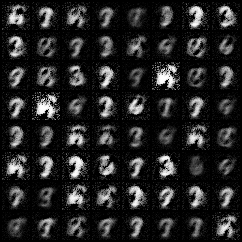
\includegraphics[width=\textwidth]{images/epoch01.png}
         \caption{Epoch: 1}
     \end{subfigure}
     \hfill
     \begin{subfigure}[b]{0.49\textwidth}
         \centering
         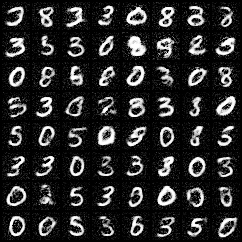
\includegraphics[width=\textwidth]{images/epoch030.png}
         \caption{Epoch: 30}
     \end{subfigure}
        \caption{Generated Images without input image normalization}
\end{figure}
As we can see there is some white noise even after 30 epochs. So I tried normalizing the input images to range $[-0.5,0.5]$.

\begin{figure}[H]
     \centering
     \begin{subfigure}[b]{0.49\textwidth}
         \centering
         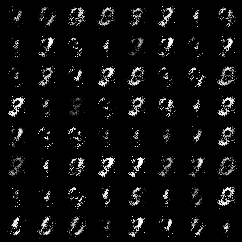
\includegraphics[width=\textwidth]{images/epoch11.png}
         \caption{Epoch: 1}
     \end{subfigure}
     \hfill
     \begin{subfigure}[b]{0.49\textwidth}
         \centering
         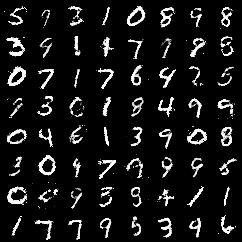
\includegraphics[width=\textwidth]{images/epoch130.png}
         \caption{Epoch: 30}
     \end{subfigure}
        \caption{Generated Images with input image normalization}
\end{figure}

\end{document}
